Actualmente existen 2 modelos InputStick: Bluetooth 2.1 y Bluetooth 4.0.\cite{stickversions} :a versión que usamos en este proyecto es la 4.0 ya que es más reciente, por ello siempre que hablemos de InputStick nos estaremos refiriendo a la versión 4.0.

InputStick es un dispositivo \gls{usb} con conexión Bluetooth. Cuando está conectado a un dispositivo mediante el puerto \gls{usb}, InputStick actúa como un periférico \gls{hid}, mientras que a través de la conexión Bluetooth se le indica a InputStick qué hacer, en nuestro caso será simular presionar las teclas de un teclado. \ref{fig:inputstick-diagram} \cite{stickworks}

\begin{figure}[H]
    \centering
    
\includegraphics[width=\textwidth]{gfx/inputstick-logo.png}
    \caption{Logo de InputStick. \href{http://inputstick.com/}{Realizado por InputStick}}
    \label{fig:inputstick-logo}
\end{figure}

\begin{figure}[H]
    \centering
    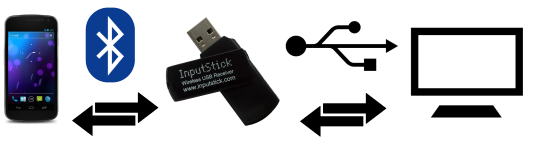
\includegraphics[width=\textwidth]{gfx/inputstick-diagram.png}
    \caption{Diagrama  de conexión InputStick. \href{http://inputstick.com/how-it-works/}{Realizado por InputStick}}
    \label{fig:inputstick-diagram}
\end{figure}
Debido a su capacidad de dispositivo \gls{hid}, InputStick puede hacerse pasar como:
\begin{itemize}
    \item \textbf{Teclado}
    \item Ratón
    \item Controlador de Videojuegos
    \item Botones multimedia
    \item Pantalla táctil
\end{itemize}

Como medida de seguridad InputStick usa conexión Bluetooth cifrada\cite{stickfaq}, además es posible activar el protocolo de cifrado \gls{aes}-128 para enviar datos, y se verificarán usando \gls{hmac}-\gls{sha}256\cite{sticksecurity}. Esta clave se puede configurar de 2 formas, ambas desde la app InputStickUtility:
\begin{itemize}
    \item De forma no segura: La clave se envía a InputStick, por lo que para ello no se puede usar una clave.
    \item De forma segura: Se le solicita a InputStick que genere una clave, InputStick procederá a escribirla en el dispositivo que se encuentre conectado, ahora el usuario la puede copiar a mano, ya que la puede ver en pantalla.
\end{itemize}

InputStick nombra a la frecuencia de reportes de escritura como velocidad, así que usaremos la misma terminología, aunque técnicamente sea incorrecto, como al hablar de la velocidad de la memoria RAM, que en realidad es frecuencia.